\documentclass[epsf,epic,eepic,eepicemu]{article} 
\oddsidemargin=-5mm
\evensidemargin=-5mm\marginparwidth=.08in \marginparsep=.01in
\marginparpush=5pt\topmargin=-15mm\headheight=12pt
\headsep=25pt
%\footheight=12pt
\footskip=30pt\textheight=25cm
\textwidth=17cm\columnsep=2mm
\columnseprule=1pt\parindent=15pt\parskip=2pt

\usepackage{amssymb,amsmath,amsthm,enumitem}
\usepackage{mathtools, bm}
\DeclareMathOperator*{\argmax}{arg\,max}
\usepackage{algorithm}
\usepackage{algpseudocode}
\usepackage{xcolor}
\usepackage[colorlinks=true,allcolors=blue]{hyperref}
\usepackage{cleveref}

\usepackage{graphicx}
\usepackage{caption}
\usepackage{subcaption}

\newcommand{\var}{\texttt}
\newcommand{\assign}{\leftarrow}
\newcommand{\multilinestate}[1]{%
  \parbox[t]{\linewidth}{\raggedright\hangindent=\algorithmicindent\hangafter=1
    \strut#1\strut}}

\begin{document}
\begin{center}
\bf Semestral project NI-PDP 2021/2022\\[5mm]
    {\Large Parallel algorithm for a maximum bipartite subgraph problem}\\[5mm]
       Anton Bushuiev\\[2mm]
Master's program, FIT CTU, Th\'akurova 9, 160 00 Praha 6\\[2mm]
\today
\end{center}

\section{Problem definition and sequential algorithm}
\label{sec:sequential}

Given an undiricted connected graph $G=(V, E)$ with non-negative edge weights $w: E \to \mathbb{N}^+$, the problem of a \textit{maximum bipartite subgraph} is to find each connected bipartite subgraph $G^*=(V^*, E^*)$ with the maximum weight among all connected bipartite subgraphs, i.e.
\begin{align}
	E^* \in \argmax_{B \subseteq E}{\sum_{e \in B}{w(e)}}.
\end{align}

The considered problem is NP-hard \cite{gutin2021} and the \textit{sequential solver} implemented in this project is a branch and bound algorithm. It is based on the fact that a graph is bipartite if and only if it can be colored with two colors. Thus, for a candidate solution $B$ the algorithm recursively tries all the possible options for each edge ${u, v} \in E$: (i) add edge to $B$ and color $u, v$ with colors $0, 1$ respectively, (ii) add edge to $B$ and color $u, v$ with colors $1, 0$ respectively and (iii)  ignore edge. While building $B$, the coloring consistency is checked and when all the edges are processed, the candidate is ready. This exhaustive search leads to $\mathcal{O}(3^{|E|})$ time complexity. To mitigate it, the implemented solver contains a simple pruning based on the sum of the weights of all yet unprocessed edges. Having such a pruning, it's rational to assume that sorting edges by their weights in descending order may reduce the algorithm's running time. Therefore, the implementation also provides this as an option. For details of the algorithm please see \Cref{alg:sequential}. The solver is implemented in C++ and can be found in \texttt{solvers/sequential.cpp}.

\section{Task-parallel algorithm and its implementation in OpenMP}

Recursive steps of the sequential algorithm generate a ternary tree.
Since the branches of a tree generated by recursion are independent, the described sequential algorithm can be easily parallelized. Thus, the idea behind the \textit{task-parallel} algorithm is that each recursive step can be treated as a separate independent task. Each thread takes one job from the common pool, performs it, and inserts up to three new ones. This process repeats for all threads until no more jobs are left and the initial computation is started by a single one. During a computation, when only a small number of edges (equal to the \var{TASK\_THRESHOLD} constant) are left unprocessed, a thread finishes them sequentially to avoid unnecessary granulation. The details of the algorithm can be found in \Cref{alg:task-parallel}.

Using OpenMP, the implementation of the task-parallel algorithm is simple. The initial computation is started using the directives \texttt{omp parallel} and \texttt{omp single}. Jobs are added to the task pool with \texttt{omp task} and the atomicity of solution update is ensured with \texttt{omp critical}. In the experiments described below, the threshold number of edges \var{TASK\_THRESHOLD} is set to 4. \texttt{solvers/task-parallel.cpp} source file contains an implementation of this algorithm.

\section{Data-parallel algorithm and its implementation in OpenMP}
\label{sec:data-parallel}

The other approach to parallelizing the sequential algorithm is to directly divide the initial tree into disjoint subtrees and process them one by one by multiple threads. The roots of subtrees can be obtained by running the breadth-first search (BFS) algorithm for some iterations and taking the content of an underlying BFS-queue. The desired number of subtrees is set as a simple function of input size: the number of edges multiplied by the constant \var{N\_JOBS\_PER\_THREAD}. Note, however, that stopping the BFS when queue size is equal to the desired number may not be possible since each search iteration adds 1 to 3 new nodes. That is why the present implementation generates at most the desired number of subtrees. \Cref{alg:data-parallel} provides a pseudo-code for the data-parallel solver.

The OpenMP-based implementation of the data-parallel algorithm is straightforward. It requires only two modifications of the sequential code. Firstly, the algorithm generates subtrees, and then they are processed in a for-loop with the directive \texttt{omp parallel for schedule(dynamic)}. Dynamic scheduling means that threads process subtrees one by one taking a new job only after finishing a previous one. For the experiments, \var{N\_JOBS\_PER\_THREAD} is set to 100. The \texttt{solvers/data-parallel.cpp} source file contains a complete implementation.

\section{Distributed algorithm and its implementation in Open MPI}

The \textit{distributed} algorithm adapts the sequential solver to run across multiple processes and threads. It is based on a master-slave approach: firstly, the master process generates jobs with the BFS algorithm, in the same way as discussed in \Cref{sec:data-parallel}. Then, it sends them one by one to free slave processes and waits for responses. In its turn, a slave process solves an assigned job with the data-parallel algorithm, sends the solution, and waits for another one until the terminal signal is not received. Again, the number of jobs constructed by the BFS depends on the constant \var{N\_JOBS\_PER\_PROCESS}. See \Cref{alg:distributed} for the details.

The implementation of this algorithm can be found in \texttt{solvers/distributed.cpp}. It utilizes an Open MPI framework for communication between processes. Serialized messages are sent and received via blocking functions \texttt{MPI\_Send} and \texttt{MPI\_Recv} through the buffer of constant size. The serialization is implemented straightforwardly using a \texttt{vector<int>} container. For all the experiments, \var{N\_JOBS\_PER\_PROCESS} for a master process and \var{N\_JOBS\_PER\_THREADS} for slave processes are both set to 10.


\section{Experiments}

\subsection*{Framework}
All the following experiments were conducted on STAR cluster (\texttt{star.fit.cvut.cz}) on NUMA nodes with 2 CPUs and 10 cores each with no hyperthreading. Therefore, the implementations of task-parallel and data-parallel algorithms were tested for 2, 4, 8, 16, and 20 threads. The implementation of a distributed MPI program was evaluated on 2, 3, and 4 nodes with 10 and 20 threads each. 

The Bash script \texttt{submit-job.sh} serves for automated testing. It generates a Sun Grid Engine (SGE) script and submits it to the cluster's queue. The script has parameters to configure a required number of processes and threads, and a type of the solver and its parameters. Executions of the script generate output files with measured jobs' running times which can be then composed into a single \texttt{.csv} file using the \texttt{compose-results.sh} script.

For the final test, 8 input graphs were generated such that the sequential algorithm solves them in 4 to 10 minutes. Namely, these are graphs of 15 to 20 nodes with either an average degree of 5 to 7 or an equal degree in the same range for each node. For the details please see \texttt{data/graphs\_final}.

\subsection*{Results}
The experimental results are visualized in \Cref{fig:results}. First of all, quite surprisingly, \Cref{fig:running-time} demonstrates that sorting edges by their weights, as discussed in \Cref{sec:sequential}, has a negative influence on running time. Then, we can observe that the task-parallel and data-parallel solvers show an expected performance: as the number of allocated threads increases, the running time decreases. \Cref{fig:acceleration} suggests that both algorithms have near-linear acceleration and the data-parallel approach consistently outperforms the task-parallel one. Moreover, the plot suggests the average lower bound on running time -- about 1 minute.

Regarding the MPI solution, the communication overhead is quite significant. Indeed, on two cores the distributed solver just ``simulates'' the data-parallel approach. However, the running time of such a simulation is the highest among all the solvers. On the other hand, the solver's performance on more than two CPUs is impressive: on three cores it already hits the estimated lower bound, and allocation of four processes leads only to a slight improvement.

Note that tuning of the constants was taken out of the project's scope despite a proper setup of their values may be crucial. Moreover, for the data-parallel and distributed algorithms, the number of subtrees is determined by a simple function dependent only on the number of available threads. The incorporation of input size may lead to better performance. Besides that, the distributed algorithm's implementation could be improved by more advanced serialization and synchronization of the best-found solutions for more efficient pruning.

\begin{figure}[htbp]
    %\centering
    \begin{subfigure}{0.3\textwidth}
        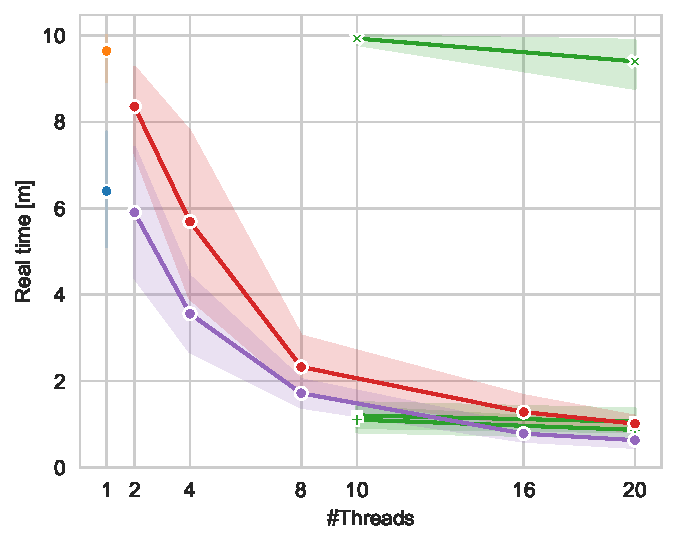
\includegraphics[height=6cm]{assets/running-time.pdf}
        \caption{Solvers' running time.}
        \label{fig:running-time}
    \end{subfigure}\hspace{2.5cm}
    \begin{subfigure}{0.3\textwidth}
        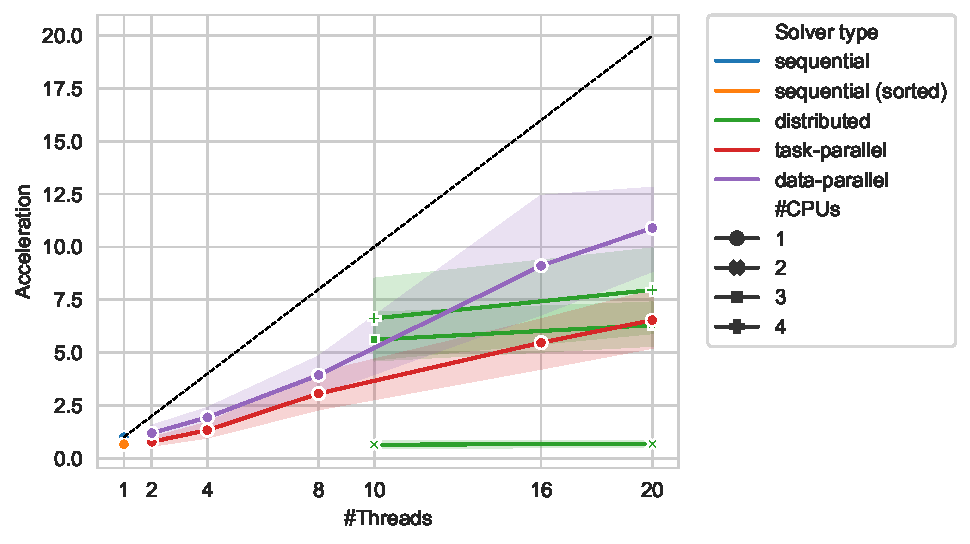
\includegraphics[height=6cm]{assets/acceleration.pdf}
        \caption{Solvers' acceleration}
        \label{fig:acceleration}
    \end{subfigure}
    \caption[Experimental results for different types of solvers.]{Experimental results for different types of solvers. The values are averages over 8 generated inputs, and margins depict standard deviation.}
    \label{fig:results}
\end{figure}

%\begin{enumerate}
%\item Zvolte tri instance problemu s takovou velikosti vstupnich dat, pro ktere ma sekvencni 
%algoritmus casovou slozitost alespon nekolik minut - vice informaci na {\tt http://courses.fit.cvut.cz} v sekci "Organizace cviceni".
%Pro mereni cas potrebny na cteni dat z disku a ulozeni na disk neuvazujte a zakomentujte
%ladici tisky, logy, zpravy a vystupy.
%\item Merte paralelni cas pri pouziti $i=2,\cdot,60$ vypocetnich jader.
%\item Tabulkova a pripadne graficky zpracovane namerene hodnoty casove slozitosti měernych instanci behu programu s popisem instanci dat. Z namerenych dat sestavte grafy zrychleni $S(n,p)$. 
%\item Analyza a hodnoceni vlastnosti paralelniho programu, zvlaste jeho efektivnosti a skalovatelnosti, pripadne popis zjisteneho superlinearniho zrychleni.
%\end{enumerate}
\section{Conclusion}

In this project, I have realized the solver for a \textit{maximum bipartite subgraph} problem in C++. Then, I implemented its three parallelizable modifications with OpenMP and Open MPI frameworks. Running on multiple threads and CPUs, they confidently and consistently outperform the original solver on randomly generated data. 

\begin{thebibliography}{10}
\bibitem{gutin2021} Gutin, Gregory and Yeo, Anders, 2021, Lower Bounds for Maximum Weighted Cut, 10.48550/ARXIV.2104.05536.
\end{thebibliography}

\begin{minipage}[t]{0.46\textwidth}
\begin{algorithm}[H]
\caption{Sequential solver}\label{alg:sequential}
\footnotesize
\begin{algorithmic}
  \State \var{SOLUTION} $\gets \emptyset$
  \newline
  \Function{BB-DFS-Sequential}{\var{edge}, \var{state}}
    \State $\var{score} \gets$ sum of \var{G} edge weights by $\var{state.edge\_mask}$
    \newline
    
    \State // Analyze state if terminal
    \If {$\var{edge} \geq |E(\var{G})|$}
      \If {$\var{G.not\_connected()}$}
        \State return
      \EndIf
      \If {$\var{SOLUTION.score} \leq \var{score}$}
        \State update $\var{SOLUTION}$ with $\var{state}$
      \EndIf
    \EndIf
    \newline
    
    \State // Prune
    \State $\var{score\_future} \gets$ sum of all $\var{G}$ weights for edges $>\var{edge}$
    \If{$\var{score} + \var{score\_future} < \var{SOLUTION.score}$}
      \State return
    \EndIf
    \newline
    
    \State // ``Ignore edge'' case
    \State $\var{state.edge\_mask}[\var{edge}] \gets$ 0
    \State \textproc{BB-DFS-Sequential}(\var{edge}+1, \var{state})
    \newline
    
    \State // ``Add edge'' cases
    \State $\var{state.edge\_mask}[\var{edge}] \gets$ 1
    \State $\var{u}, \var{v} \gets \var{G.edges[edge]}$
    \For{\var{colors} in $\{(0, 1), (1, 0)\}$}
      \If{$\var{state.colors[u]} \neq \var{colors[0]}$ \\ \hskip\algorithmicindent\hskip\algorithmicindent or $\var{state.colors[v]} \neq \var{colors[1]}$}
        \State continue
	  \EndIf
      \State $\var{state.colors[u]} \gets \var{colors[0]}$
      \State $\var{state.colors[v]} \gets \var{colors[1]}$
      \If{coloring in \var{state} is consistent}
        \State \textproc{BB-DFS-Sequential}(\var{edge}+1, \var{state})
      \EndIf
    \EndFor
  
  \EndFunction
  \newline
  \Function{Main}{\var{infile}, \var{sort}}
  	\State $\var{G} \gets$ parse \var{infile}
    \If{$\var{G}$ is bipartite}
      \State \var{SOLUTION} $\gets \{\var{G}\}$
      \State print \var{SOLUTION} and exit
    \EndIf
    \If{$\var{sort}$ is True}
      \State Sort edges of \var{G} by weights
    \EndIf
    \State \textproc{BB-DFS-Sequential}(0, $\emptyset$)
    \State print \var{SOLUTION} and exit
  \EndFunction
  
\end{algorithmic}
\end{algorithm}
\end{minipage}
\hfill
\begin{minipage}[t]{0.46\textwidth}
\begin{algorithm}[H]
\caption{Task-parallel solver}\label{alg:task-parallel}
\footnotesize
\begin{algorithmic}
  
  \State \var{SOLUTION} $\gets \emptyset$
  \newline
  \Function{\textcolor{red}{BB-DFS-Task}}{\var{edge}, \var{state}}
    \State $\var{score} \gets$ sum of \var{G} edge weights by $\var{state.edge\_mask}$
    \newline
    
    \State // Analyze state if terminal
    \If {$\var{edge} \geq |E(\var{G})|$}
      \If {$\var{G.not\_connected()}$}
        \State return
      \EndIf
      \State \textcolor{red}{Critical section \{}
      \If {$\var{SOLUTION.score} \leq \var{score}$}
        \State update $\var{SOLUTION}$ with $\var{state}$
      \EndIf
      \State \textcolor{red}{\}}
    \EndIf
    \newline
    
    \State // Prune
    \State $\var{score\_future} \gets$ sum of all $\var{G}$ weights for edges $>\var{edge}$
    \If{$\var{score} + \var{score\_future} < \var{SOLUTION.score}$}
      \State return
    \EndIf
    \newline
    
    \State // ``Ignore edge'' case
    \State $\var{state.edge\_mask}[\var{edge}] \gets$ 0
    \If{coloring in \var{state} is consistent}
        \textcolor{red}{
        \If{$|E(\var{G})| - 1 - \var{edge} > \var{TASK\_THRESHOLD}$}
          \State Add task ``\textproc{BB-DFS-Task}(\var{edge}+1,\var{state})''
        \Else 
          \State \textproc{BB-DFS-Task}(\var{edge}+1, \var{state})
        \EndIf
        }
    \EndIf
    \newline
    
    \State // ``Add edge'' cases
    \State $\var{state.edge\_mask}[\var{edge}] \gets$ 1
    \State $\var{u}, \var{v} \gets \var{G.edges[edge]}$
    \For{\var{colors} in $\{(0, 1), (1, 0)\}$}
      \If{$\var{state.colors[u]} \neq \var{colors[0]}$ \\ \hskip\algorithmicindent\hskip\algorithmicindent or $\var{state.colors[v]} \neq \var{colors[1]}$}
        \State continue
	  \EndIf
      \State $\var{state.colors[u]} \gets \var{colors[0]}$
      \State $\var{state.colors[v]} \gets \var{colors[1]}$
      \If{coloring in \var{state} is consistent}
        \textcolor{red}{
        \If{$|E(\var{G})| - 1 - \var{edge} > \var{TASK\_THRESHOLD}$}
          \State Add task ``\textproc{BB-DFS-Task}(\var{edge}+1,\var{state})''
        \Else 
          \State \textproc{BB-DFS-Task}(\var{edge}+1, \var{state})
        \EndIf
        }
      \EndIf
    \EndFor
  \EndFunction
  \newline
  
  \Function{Main}{\var{infile}, \var{sort}}
  	\State $\var{G} \gets$ parse \var{infile}
    \If{$\var{G}$ is bipartite}
      \State \var{SOLUTION} $\gets \{\var{G}\}$
      \State print \var{SOLUTION} and exit
    \EndIf
    \If{$\var{sort}$ is True}
      \State Sort edges of \var{G} by weights
    \EndIf

    \State \textcolor{red}{Run by single thread \{}
    \State \hskip\algorithmicindent\textproc{BB-DFS-Task}(0, $\emptyset$)
    \State \textcolor{red}{\}}

    \State print \var{SOLUTION} and exit
  \EndFunction
  
\end{algorithmic}
\end{algorithm}
\end{minipage}

\begin{minipage}[t]{0.46\textwidth}
\begin{algorithm}[H]
\caption{Data-parallel solver}\label{alg:data-parallel}
\footnotesize
\begin{algorithmic}
  \State \var{SOLUTION} $\gets \emptyset$
  \newline
  \Function{\textcolor{red}{BB-DFS-Data}}{\var{edge}, \var{state}}
    \State $\var{score} \gets$ sum of \var{G} edge weights by $\var{state.edge\_mask}$
    \newline
    
    \State // Analyze state if terminal
    \If {$\var{edge} \geq |E(\var{G})|$}
      \If {$\var{G.not\_connected()}$}
        \State return
      \EndIf
      \State \textcolor{red}{Critical section \{}
      \If {$\var{SOLUTION.score} \leq \var{score}$}
        \State update $\var{SOLUTION}$ with $\var{state}$
      \EndIf
      \State \textcolor{red}{\}}
    \EndIf
    \newline
    
    \State // Prune
    \State $\var{score\_future} \gets$ sum of all $\var{G}$ weights for edges $>\var{edge}$
    \If{$\var{score} + \var{score\_future} < \var{SOLUTION.score}$}
      \State return
    \EndIf
    \newline
    
    \State // ``Ignore edge'' case
    \State $\var{state.edge\_mask}[\var{edge}] \gets$ 0
    \State \textproc{\textcolor{red}{BB-DFS-Data}}(\var{edge}+1, \var{state})
    \newline
    
    \State // ``Add edge'' cases
    \State $\var{state.edge\_mask}[\var{edge}] \gets$ 1
    \State $\var{u}, \var{v} \gets \var{G.edges[edge]}$
    \For{\var{colors} in $\{(0, 1), (1, 0)\}$}
      \If{$\var{state.colors[u]} \neq \var{colors[0]}$ \\ \hskip\algorithmicindent\hskip\algorithmicindent or $\var{state.colors[v]} \neq \var{colors[1]}$}
        \State continue
	  \EndIf
      \State $\var{state.colors[u]} \gets \var{colors[0]}$
      \State $\var{state.colors[v]} \gets \var{colors[1]}$
      \If{coloring in \var{state} is consistent}
        \State \textproc{\textcolor{red}{BB-DFS-Data}}(\var{edge}+1, \var{state})
      \EndIf
    \EndFor
  
  \EndFunction
  \newline
  \Function{Main}{\var{infile}, \var{sort}}
  	\State $\var{G} \gets$ parse \var{infile}
    \If{$\var{G}$ is bipartite}
      \State \var{SOLUTION} $\gets \{\var{G}\}$
      \State print \var{SOLUTION} and exit
    \EndIf
    \If{$\var{sort}$ is True}
      \State Sort edges of \var{G} by weights
    \EndIf
    \State \textcolor{red}{\var{n\_jobs} $\gets \var{N\_THREADS} * \var{N\_JOBS\_PER\_THREAD}$}
    \State \textcolor{red}{\var{jobs} $\gets$ generate \var{n\_jobs} jobs with BFS}
    \State \textcolor{red}{Run \textbf{for} in parallel with \textit{dynamic} scheduler \{}
    \For{\textcolor{red}{\var{job} in \var{jobs}}}
      \State\textcolor{red}{\hskip\algorithmicindent\textproc{BB-DFS-Data}(\var{job.edge}, \var{job.state})}
    \EndFor
    \State \textcolor{red}{\}}
    \State print \var{SOLUTION} and exit
  \EndFunction
\end{algorithmic}
\end{algorithm}
\end{minipage}
\hfill
\begin{minipage}[t]{0.46\textwidth}
\begin{algorithm}[H]
\caption{Distributed solver}\label{alg:distributed}
\footnotesize
\begin{algorithmic}
  \State \var{SOLUTION} $\gets \emptyset$
  \newline
  
  \Function{Main}{\var{infile}, \var{sort}}
  	\State $\var{G} \gets$ parse \var{infile}
  	\If{Master process and $\var{G}$ is bipartite}
        \State \var{SOLUTION} $\gets \{\var{G}\}$
        \State Send terminate signal to all other processes
        \State print \var{SOLUTION} and exit
    \EndIf
    \If{$\var{sort}$ is True}
      \State Sort edges of \var{G} by weights
    \EndIf
    \newline
    \If{Master process}
      \State \var{n\_jobs} $\gets \var{N\_PROCESSES} * \var{N\_JOBS\_PER\_PROCESS}$
      \State \var{jobs} $\gets$ generate \var{n\_jobs} jobs with BFS
      \State \var{n\_workers} $\gets$ \var{N\_PROCESSES}
      \State Send one job to all other processes
      \While {$\var{n\_workers} > 0$}
        \State \var{solution} $\gets$ receive from some other \var{proc}
        \If {\var{jobs} is not empty}
          \State Send next job to \var{proc}
        \Else
          \State Send terminate signal to \var{proc}
          \State $\var{n\_workers}--$
        \EndIf
        \State \var{SOLUTION}.update(\var{solution})
      \EndWhile
      \State print \var{SOLUTION} and exit
    \newline
    \Else
      \While{True}
        \State \var{msg} $\gets$ receive from master process
        \If{\var{msg} is job}
          \State Solve \var{job} with data-parallel algorithm
          \State Send \var{SOLUTION} to master process
        \Else
          \State Break
        \EndIf
      \EndWhile
    \EndIf
  \EndFunction
\end{algorithmic}
\end{algorithm}
\end{minipage}

\end{document}
